
\documentclass[journal,transmag]{IEEEtran}
\hyphenation{op-tical net-works semi-conduc-tor}

\usepackage{enumitem}

% *** GRAPHICS RELATED PACKAGES ***
%
\ifCLASSINFOpdf
   \usepackage[pdftex]{graphicx}
  % declare the path(s) where your graphic files are
  % \graphicspath{{../pdf/}{../jpeg/}}
  % and their extensions so you won't have to specify these with
  % every instance of \includegraphics
  % \DeclareGraphicsExtensions{.pdf,.jpeg,.png}
\else
  % or other class option (dvipsone, dvipdf, if not using dvips). graphicx
  % will default to the driver specified in the system graphics.cfg if no
  % driver is specified.
  % \usepackage[dvips]{graphicx}
  % declare the path(s) where your graphic files are
  % \graphicspath{{../eps/}}
  % and their extensions so you won't have to specify these with
  % every instance of \includegraphics
  % \DeclareGraphicsExtensions{.eps}
\fi
% graphicx was written by David Carlisle and Sebastian Rahtz. It is
% required if you want graphics, photos, etc. graphicx.sty is already
% installed on most LaTeX systems. The latest version and documentation
% can be obtained at: 
% http://www.ctan.org/pkg/graphicx
% Another good source of documentation is "Using Imported Graphics in
% LaTeX2e" by Keith Reckdahl which can be found at:
% http://www.ctan.org/pkg/epslatex
%
% latex, and pdflatex in dvi mode, support graphics in encapsulated
% postscript (.eps) format. pdflatex in pdf mode supports graphics
% in .pdf, .jpeg, .png and .mps (metapost) formats. Users should ensure
% that all non-photo figures use a vector format (.eps, .pdf, .mps) and
% not a bitmapped formats (.jpeg, .png). The IEEE frowns on bitmapped formats
% which can result in "jaggedy"/blurry rendering of lines and letters as
% well as large increases in file sizes.
%
% You can find documentation about the pdfTeX application at:
% http://www.tug.org/applications/pdftex





\begin{document}

\title{\textsc{Capacidades Caloríficas}}

\author{
\IEEEauthorblockN{David S. Castro , William A. Gómez,  Ana M. Niño, Laura V. Pachón , Juliana Ramos y Luis A. Cañón,}
\IEEEauthorblockA{Pontificia Universidad Javeriana, Bogotá, Colombia}
\IEEEauthorblockA{Informe de laboratorio de Capacidades Caloríficas}
\IEEEauthorblockA{Grupo I}

}
% The paper headers
\markboth{Capacidades Caloríficas. Octubre 13~2021}%
{Shell \MakeLowercase{\textit{et al.}}: Bare Demo of IEEEtran.cls for IEEE Transactions on Magnetics Journals}
\IEEEtitleabstractindextext{%

	\begin{abstract}
	
	\end{abstract}
	\begin{IEEEkeywords}
	
	 	\end{IEEEkeywords}}


\maketitle
\IEEEdisplaynontitleabstractindextext
\IEEEpeerreviewmaketitle


\section{Resumen}



\section{Introduction}
	
	
	
	\begin{enumerate}
	
  \item Baño termostatado: Se utiliza para elevar la temperatura del agua.

		\begin{figure}[!h]
			\center
			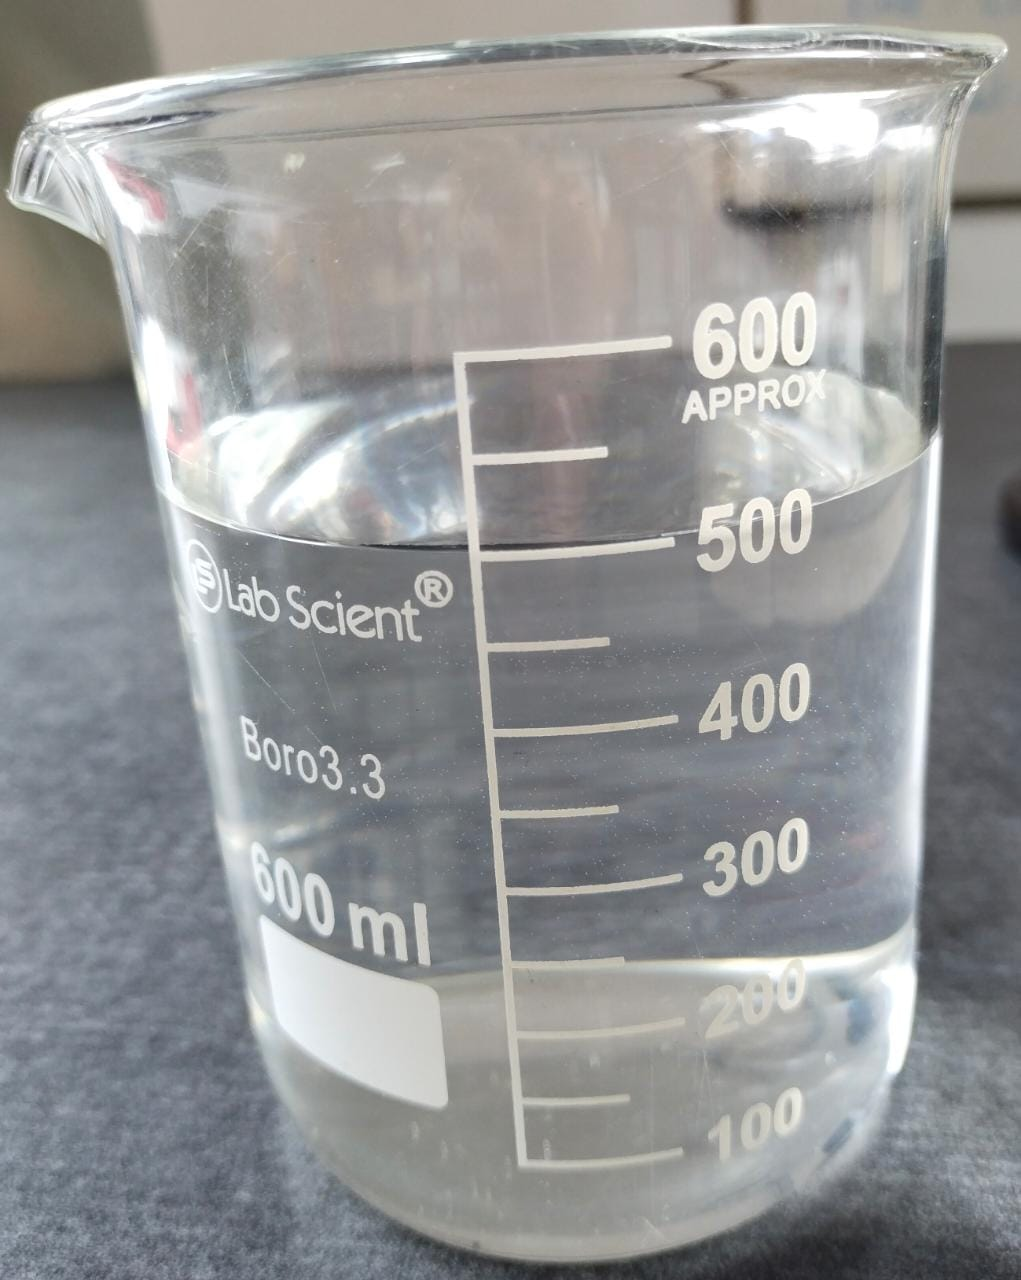
\includegraphics[width=3cm]{img/agua.jpeg}
			\caption{200 mL de Agua}
			\label{f1}
		\end{figure}
  \item Dilatómetro: Se utiliza para registrar el cambio de longitud de la varilla
		\begin{figure}[!h]
			\center
			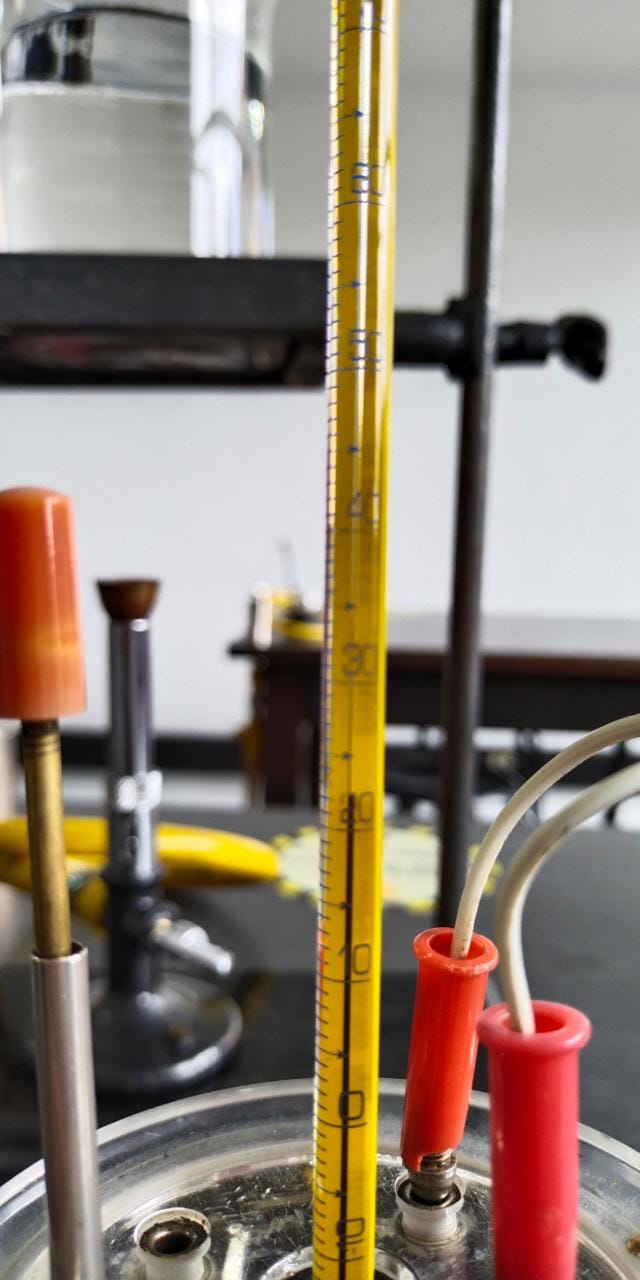
\includegraphics[width=3cm]{img/termometro.jpeg}
			\caption{Termómetro.}
			\label{f2}
		\end{figure}
  \item Termómetro: Se utiliza para registrar los cambios de temperatura en el agua
		\begin{figure}[!h]
			\center
			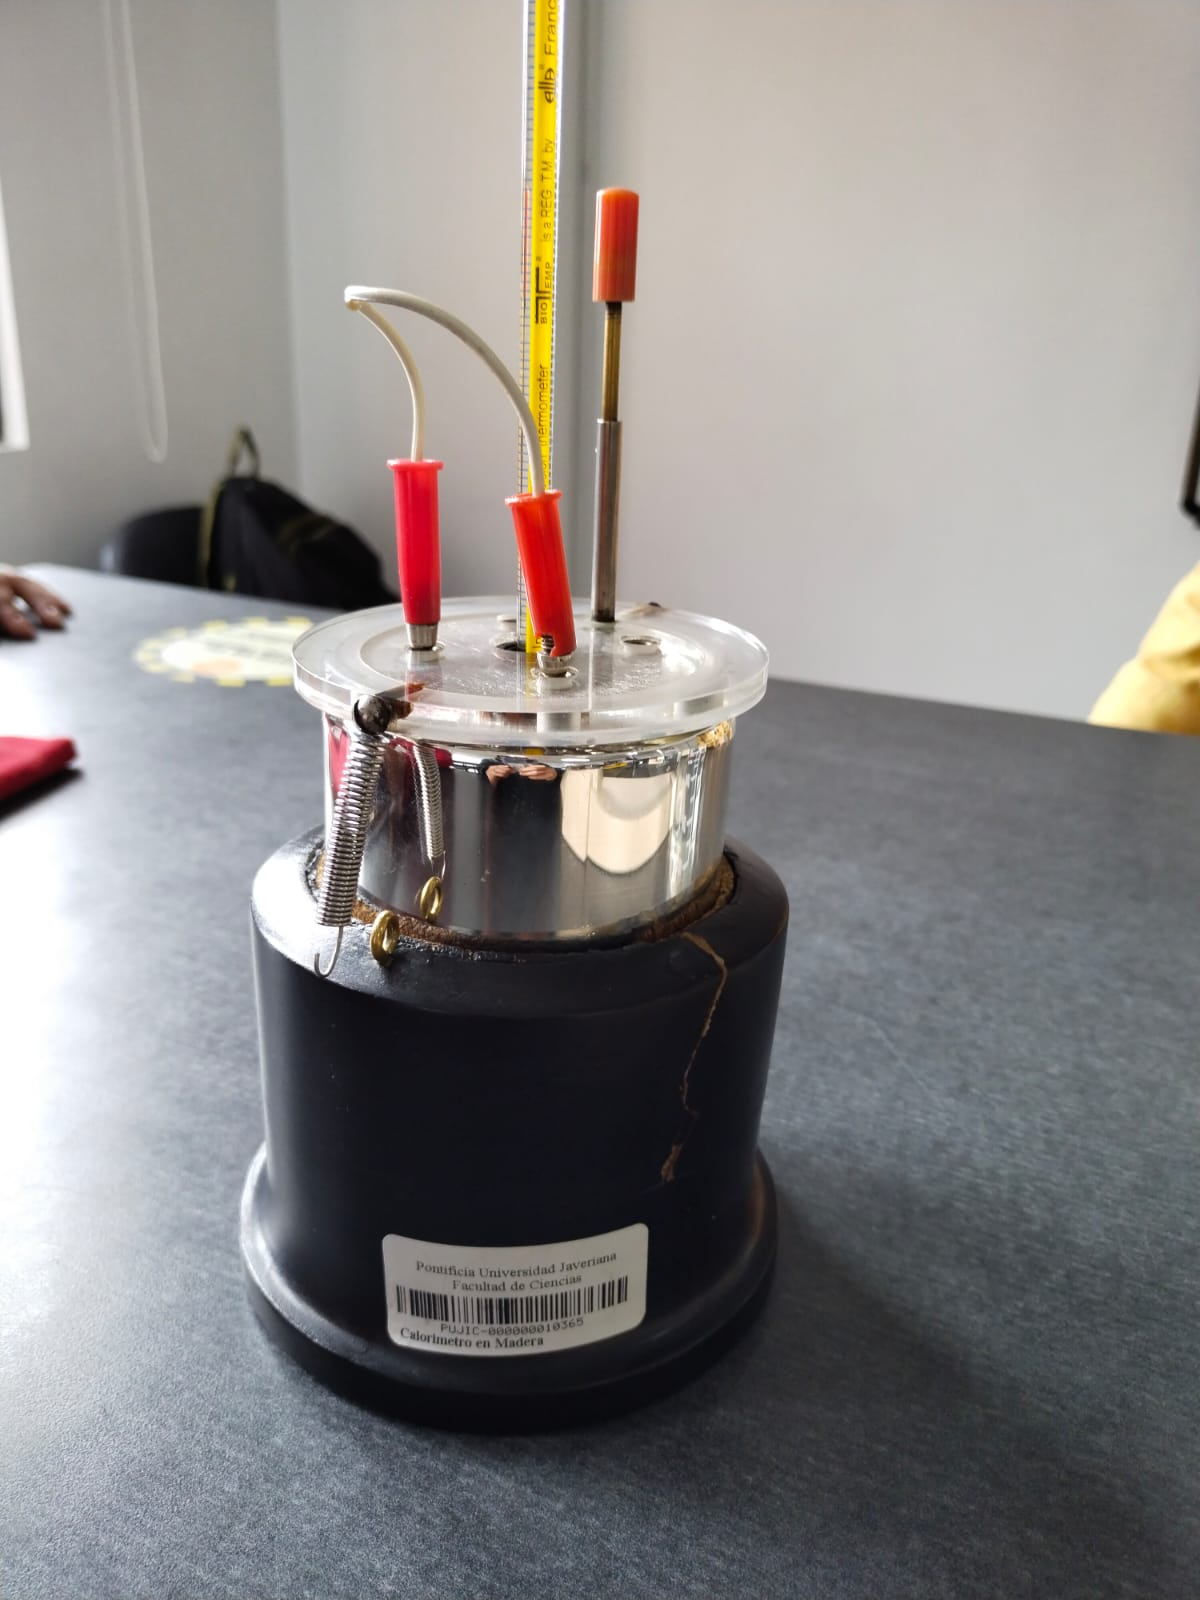
\includegraphics[width=4cm]{img/calorimetro.jpeg}
			\caption{Calorímetro}
			\label{f3}
		\end{figure}
 \item Se utiliza para determinar la longitud inicial de la varilla
			\begin{figure}[!h]
				\center
				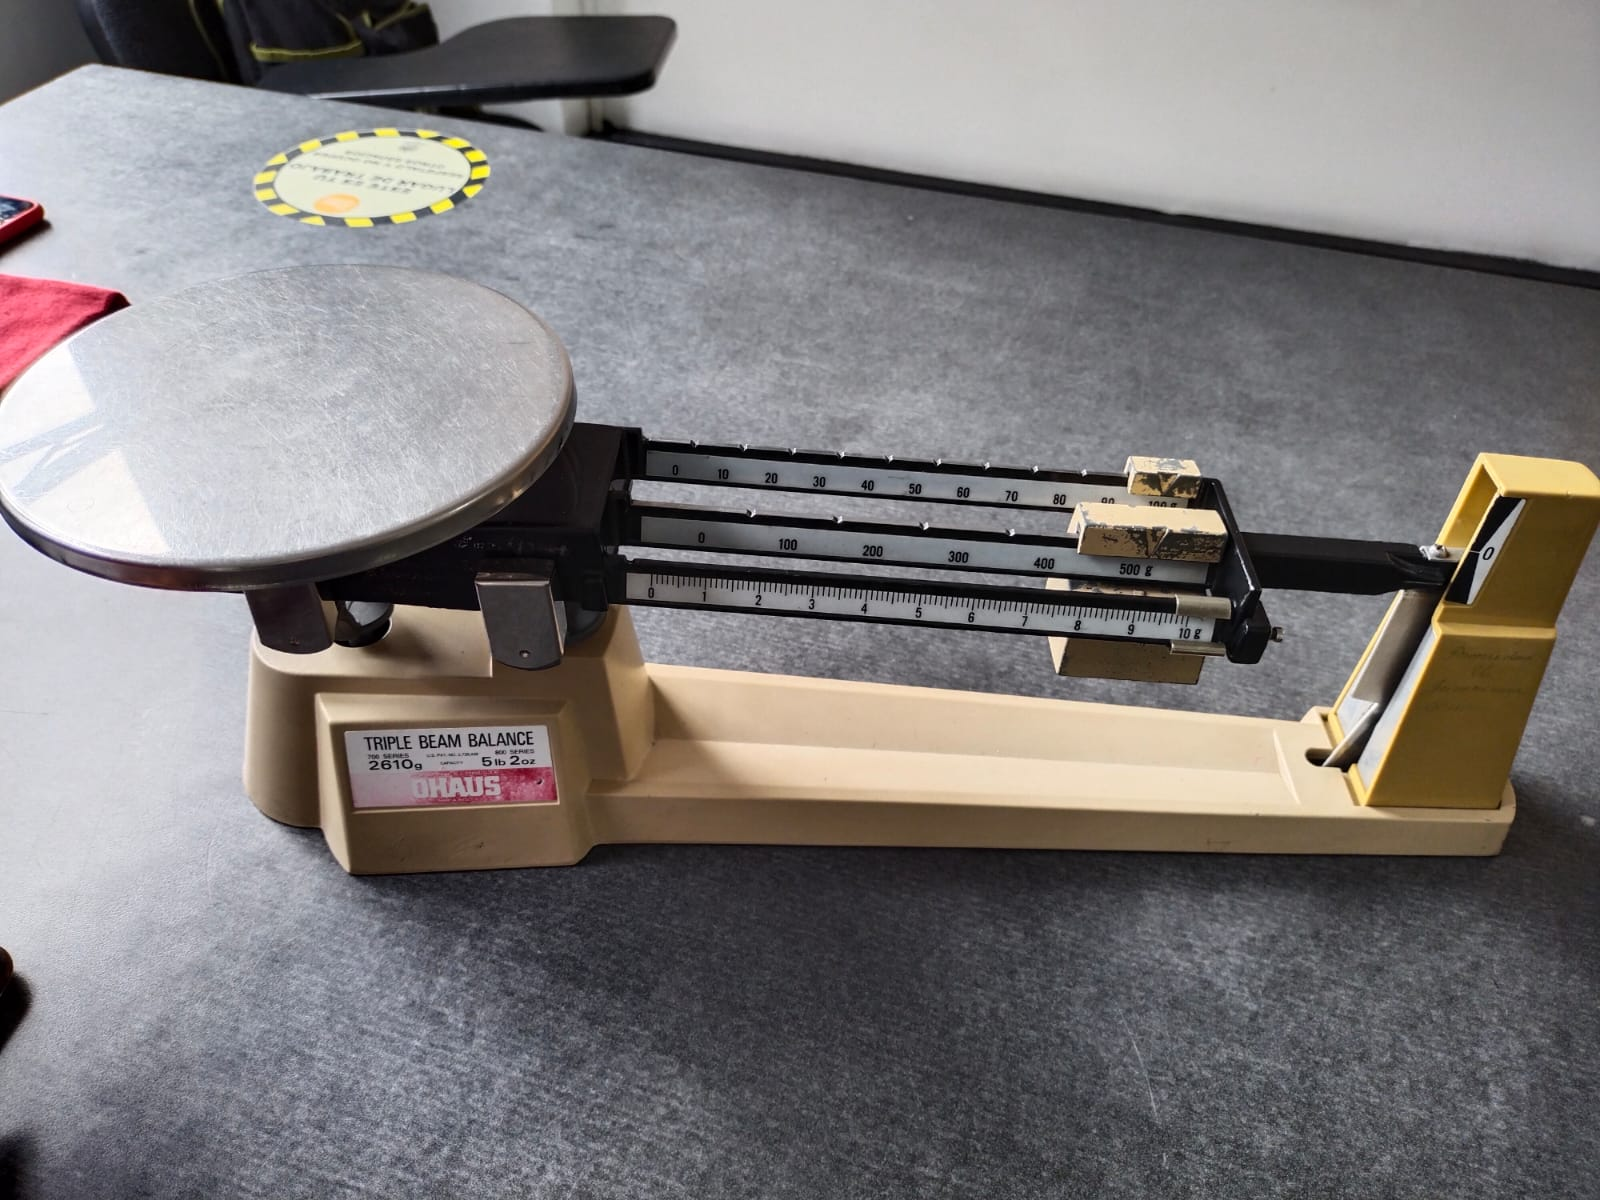
\includegraphics[width=6cm]{img/pesa.jpeg}
				\caption{Balanza}
				\label{f4}
			\end{figure}


	\end{enumerate}


%%%%%%%%%%%%%%%%%%%%%%%%%%OBJETIVOS
\section{Objetivos}

	\begin{enumerate}
		\item Entender la noción de calor.
		\item Utilizar el primer principio de la termodinámica.
		\item Diferenciar entre variables de estado y variables de proceso.
		\item Poder calcular capacidades caloríficas y calores específicos de diferen-
	tes sistemas. 
	\end{enumerate}
%%%%%%%%%%%%%%%%%%%%%%%%%%MARCO TEÓRICO
\section{Marco Teórico}

 
 

 
%%%%%%%%%%%%%%%%%%%%%%%%%%RESULTADOS
\section{Resultados} 


\vspace{20mm}
\begin{table}[!h] 
	\center 
	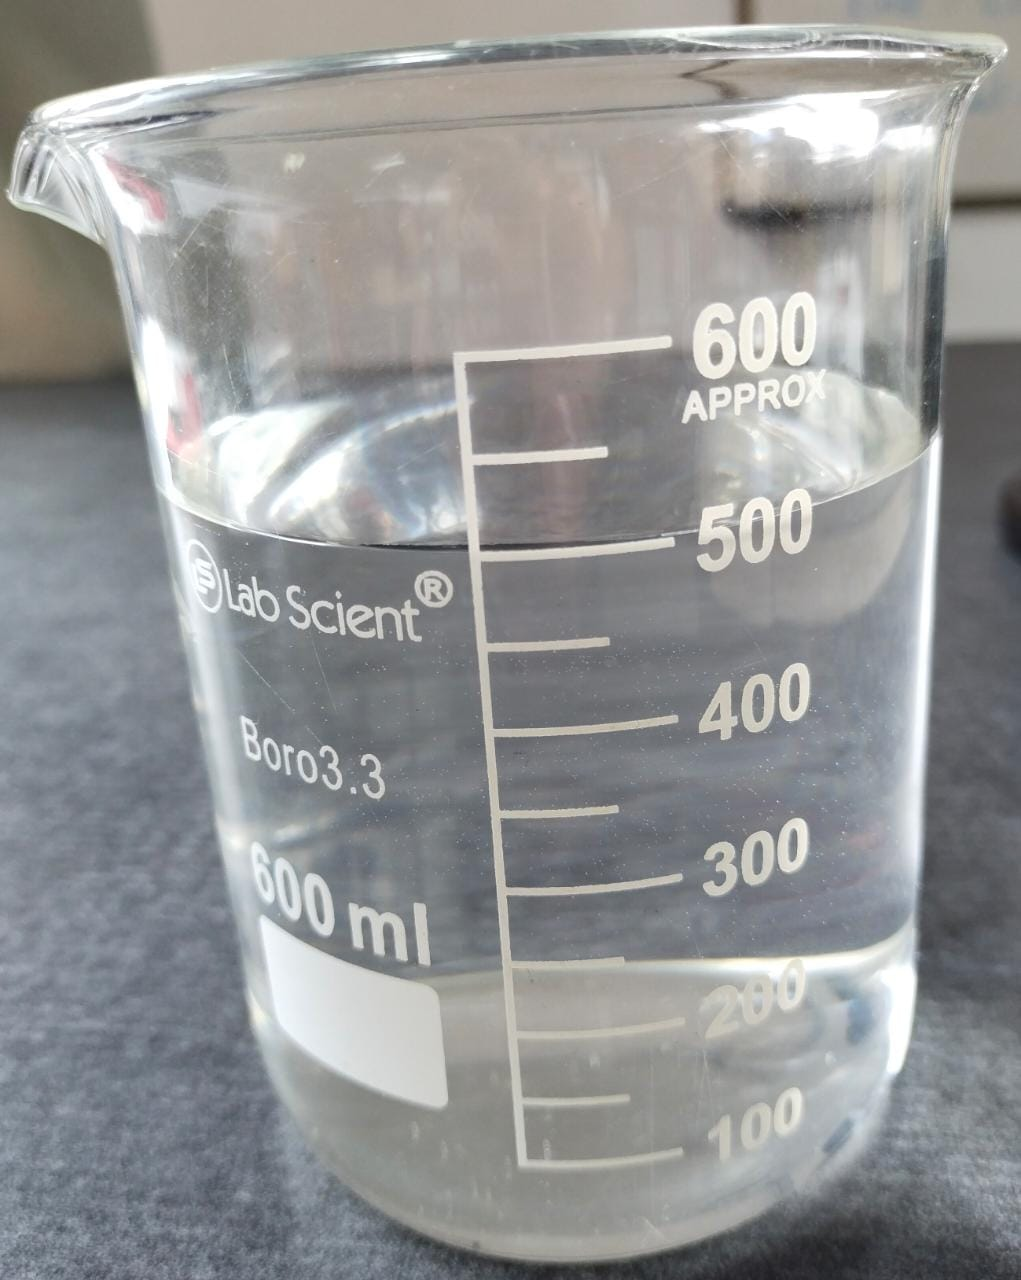
\includegraphics[width=4cm]{img/agua.jpeg} 
	\caption{Datos registrados: Medidas del laboratorio} 
	\label{T4} 
\end{table} 


%%%%%%%%%%%%%%%%%%%%%%%%%%%%%%%%%%%%%%%%%%%%%%%%%%%%RESULTADOS

\section{Análisis de resultados}


\section{Conclusion}
	
	\begin{enumerate}[label=(\roman*)]
		\item 
		\item    
		\item  
	\end{enumerate}

\appendices


\ifCLASSOPTIONcaptionsoff
  \newpage
\fi


\begin{thebibliography}{1}


 \bibitem{IEEEhowto:Monteria}
  F 

 \bibitem{IEEEhowto:Monteria}
 L
\end{thebibliography}



\end{document}
